% (C) Marc Lijour, 2016-2017 
% Licensed under a Creative Commons License BY-SA
% https://creativecommons.org/licenses/by-sa/2.5/ca/
% Presentation for the Toronto Odoo Meetup May 24, 2017
% see https://www.meetup.com/Odoo-Toronto/events/239219681/?eventId=239219681
% authored by Marc Lijour, May 2017
% 
% Variables
% TODO set the variables
% ---------------------- USER-DEFINED --------------------------------
\newcommand{\SFLtitle}{Discover~Odoo}
\newcommand{\SFLlongtitle}{Business Digitization made easy with Odoo}
\newcommand{\SFLsubtitle}{Special Odoo Toronto Meetup @ Brightlane (June 2017)}
\newcommand{\SFLauthor}{Marc~Lijour}
\newcommand{\SFLdate}{June~28, 2017}
\newcommand{\SFLsubject}{Odoo}
% --------------------------------------------------------------------
% Template
\input{../templates/sfl-presentation-template-blue-EN-with-CC-BY-SA}
% Extra packages
\usepackage{amssymb}
\usepackage{amsmath}
\usepackage[american]{babel}
\usepackage{csquotes}
\usepackage[backend=biber,style=apa]{biblatex}
\DeclareLanguageMapping{american}{american-apa}
% Use one bib file per section
%\addbibresource{references-program-overview.bib}
\addbibresource{references-odoo-course-erp.bib}
\definecolor{links}{HTML}{2A1B81}
\hypersetup{colorlinks,linkcolor=,urlcolor=links}
% Start of the document
\begin{document}
% Cover page
% Do not use this: \frame{\titlepage}
% use this instead:
\SFLcoverpage

% ======================================================================================================
%                                     Setting the stage
% ======================================================================================================
\section{Introduction}
\frame{
	\frametitle{Presenters}
	We are your neighbours at Brightlane!
	\vspace{1.5em}
	\begin{block}{Marc Lijour, Savoir-faire Linux}
		Business Digitization Consultant helping organizations use technology to make their lives easier and their business more impactful.\\
		\vspace{.5em}\tiny{Other Board \& Advisory roles @ ICTC, ColliderX, Toronto French Business Network, Techweek, Prepr}
	\end{block}
	\begin{alertblock}{Daniel Dico, OERP Canada}
		Founder @ OERP Canada and Consultant\\
		Odoo expert
	\end{alertblock}
}

\frame{
	\frametitle{Agenda}
	This \href{https://www.meetup.com/Odoo-Toronto/events/240271884/}{special session at Brightlane} of the Odoo Toronto meetup group has 2 main objectives:
	\begin{enumerate}
		\item Introducing the Brightlane community to our work with Business Digitization and why we use Odoo %: an All-in-One Management Software, Beautiful and Easy to Use
		\item Presenting the Odoo community
	\end{enumerate}
}
% ======================================================================================================
%                                     Odoo: What is it?
% ======================================================================================================
\section{Odoo in two words}
% --------------------- Short intro --------------------------
\subsection{Smart and Simple}
\frame{ % Problem statement
	\frametitle{Digitization: our \#1 business challenge}
	Troubling facts:
	\begin{itemize}
		\item Canada gets a D mark on productivity
		\item 40\% of Ontario businesses lack an Internet presence
		\item Adoption of technology is slow 
	\end{itemize}
}

\frame{
	\frametitle{How can technology help?}
	\centering
	\Huge{Automate, Assist, Amplify}
}

\frame{
	\frametitle{Why aren't we there yet?}
	\begin{itemize}
		\item Complexity
		\pause
		\item Cost
		\pause
		\item Lack of choice
		\pause
		\item Long and cumbersome implementation process
	\end{itemize}
}

\frame{
	\frametitle{A business owner conundrum}
	How do I choose between
	\begin{itemize}
		\item a complex system that does everything but expensive in terms of raw dollars and time to implement?
		\item smarter and leaner systems very good in their niche, but exponentially difficult to integrate to fit the business needs?
	\end{itemize}
}

\frame{
	\frametitle{A Short Introduction to Odoo}
	\framesubtitle{Odoo in a few words}
	\begin{figure}	
		\centering
		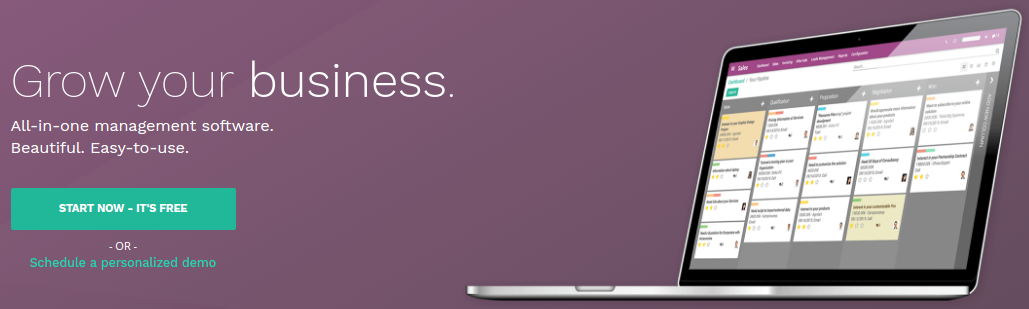
\includegraphics[width=12cm]{../pics/odoo-tagline}
		\caption{\url{https://www.odoo.com} (\cite{odoosa})}
	\end{figure}
}

\frame{
	\frametitle{An Operating System for Small Business}
	\framesubtitle{The Fun way to doing more, faster, better, and cheaper...}
	\begin{figure}
	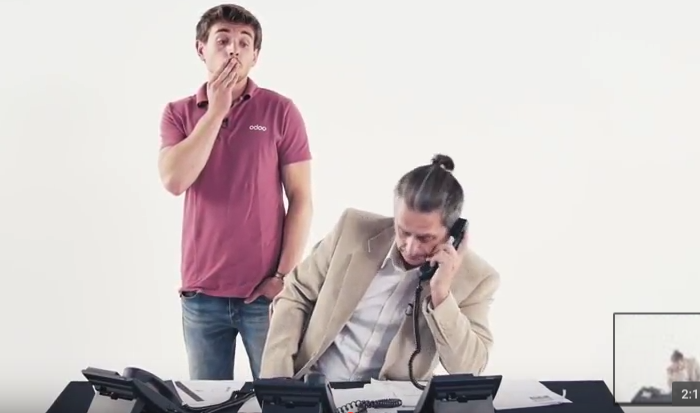
\includegraphics[width=11.5cm]{../pics/odoo-youtube-notERP}
	\caption{\tiny\url{https://www.youtube.com/watch?v=2dhyhamLm6M&list=PL1-aSABtP6AALA_4hW2TyYIioOVEGQ3yf&index=6}}
	\end{figure}
}

%\frame{
%	\frametitle{}
%	\framesubtitle{}
%}

\frame{
	\frametitle{A Short Introduction to Odoo}
	\framesubtitle{Value Proposition}
	\begin{figure}	
		\centering
		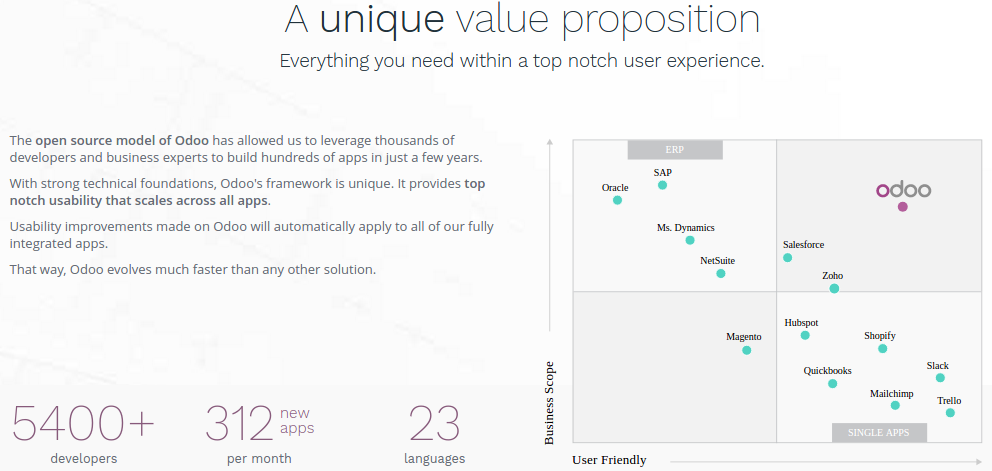
\includegraphics[width=12cm]{../pics/odoo-unique-value-prop}
	\end{figure}
}

\frame{
	\frametitle{Better, Faster, Cheaper}
	\begin{figure}	
		\centering
		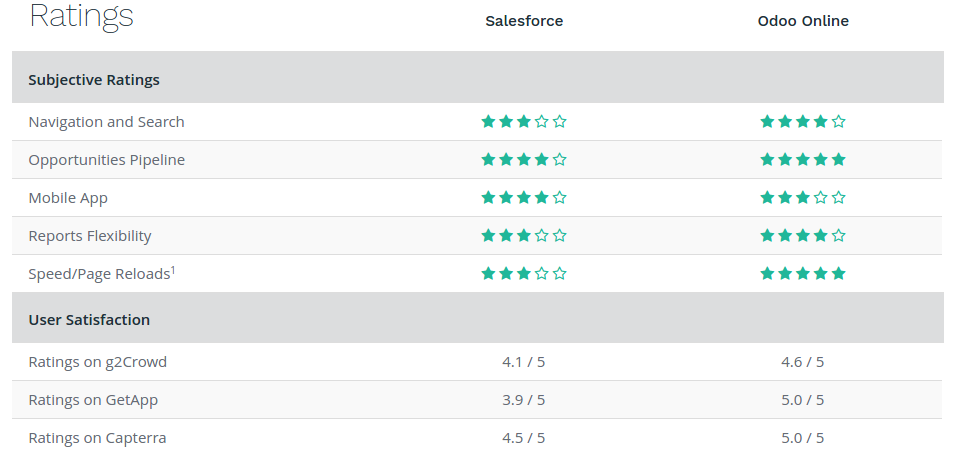
\includegraphics[width=11.5cm]{../pics/odoo-vs-sfdc-ux}
		\caption{Better UX can also be 5x cheaper, see \href{https://www.odoo.com/page/compare-odoo-vs-salesforce}{Odoo vs. Saleforce}}
	\end{figure}
}

\frame{
	\frametitle{\emph{Great User Experience Award} and the \emph{2017 Rising Star}}
	\begin{figure}	
		\centering
		
\includegraphics[width=12cm]{../pics/odoo-awards2017}
		\caption{\href{https://www.odoo.com/blog/odoo-news-5/post/odoo-wins-two-prestigious-erp-software-awards-from-financesonline-362}{Odoo News April 2017}}
	\end{figure}
}

\frame{
	\frametitle{Odoo is growing faster than Salesforce}
	\begin{figure}	
		\centering
		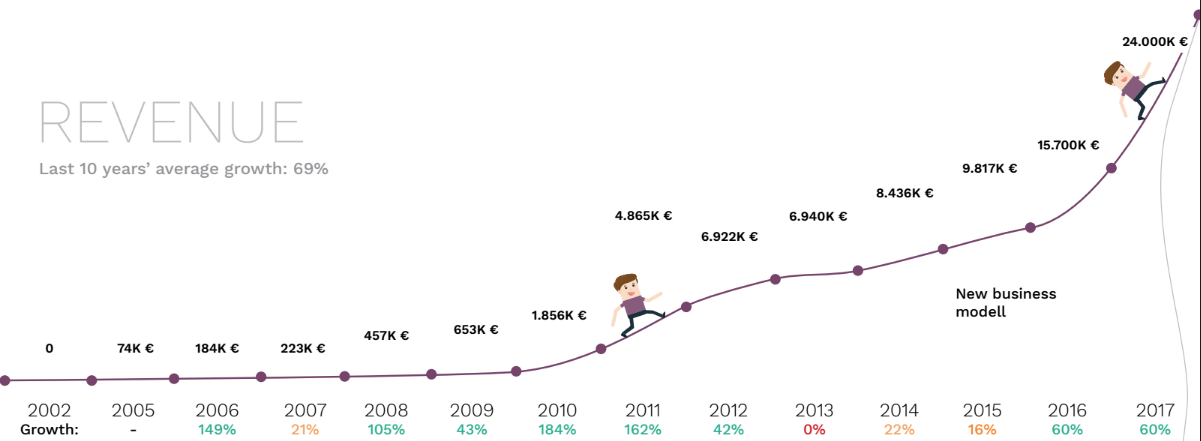
\includegraphics[width=12cm]{../pics/odoo-revenue-growth}
		\caption{Odoo Revenue Growth, available at \url{http://bit.ly/2pnexIa} --tweeted by Fabien Pinckaers (@fpodoo) April 14, 2017}
	\end{figure}
}

\frame{
	\frametitle{Odoo is growing faster than Salesforce}
	\begin{figure}	
		\centering
		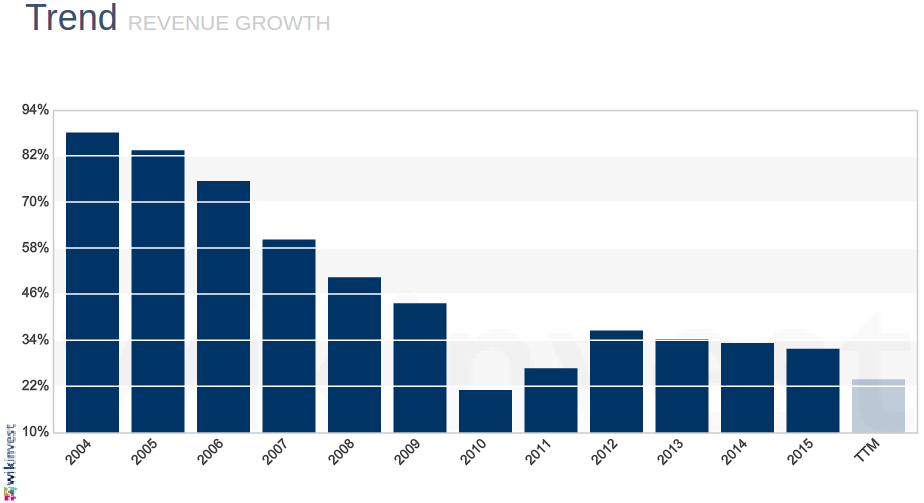
\includegraphics[height=6cm]{../pics/wikinvest-SFDC-revenue-growth}
		\caption{Salesforce (SFDC) Revenue Growth from \href{http://www.wikinvest.com/stock/Salesforce.com_(CRM)/Data/Revenue_Growth}{wikinvest} \\\footnotesize{\emph{(started in 1999, SFDC raised US\$110 million in its June 2004 IPO)}}}
	\end{figure}
}

\frame{
	\frametitle{Odoo is a great deal}
	\begin{itemize}
		\item US\$1 a day per user 
		\pause
		\item Buffet-style access to all apps in Enterprise edition
		\pause
		\item ``App store'' with \href{https://www.odoo.com/blog/odoo-news-5/post/10000-apps-in-the-odoo-app-store-352}{more than 10,000 integrated apps}\\(86\% Open Source) after 2 years of existence
		\pause
		\item Odoo SA is operating in 100 countries
		\pause
		\item Free/Free Community version (ability to innovate)
		\pause
		\item A fairly good \href{https://www.odoo.com/partners/country/canada-36}{Odoo partner ecosystem} in Canada
	\end{itemize}
}

\frame{
	\frametitle{Thousands of free apps curated by the Odoo Communication Association (OCA)}
	\begin{figure}	
		\centering
		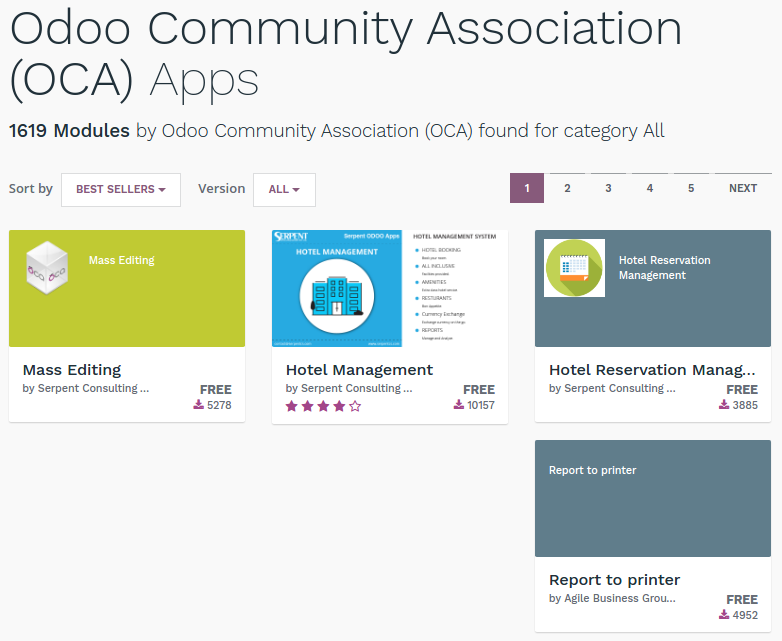
\includegraphics[height=6cm]{../pics/odoo-OCA-apps}
		\caption{See the \href{https://www.odoo.com/apps/modules?author=Odoo\%20Community\%20Association\%20(OCA)}{OCA section on Odoo.com} and \url{https://github.com/OCA} (\cite{ocagithub,ocaappsonodoo})}
	\end{figure}
}

% --------------------- For Developers --------------------------
\subsection{The pitch to Developers}
\frame{
	\frametitle{The pitch to developers}
	\centering
	\Huge{Odoo is a modern,\\extensible platform,\\with a lively community}
}

\frame{
	\frametitle{It's easy to create Apps (even for non-developers)}
	\begin{figure}	
		\centering
		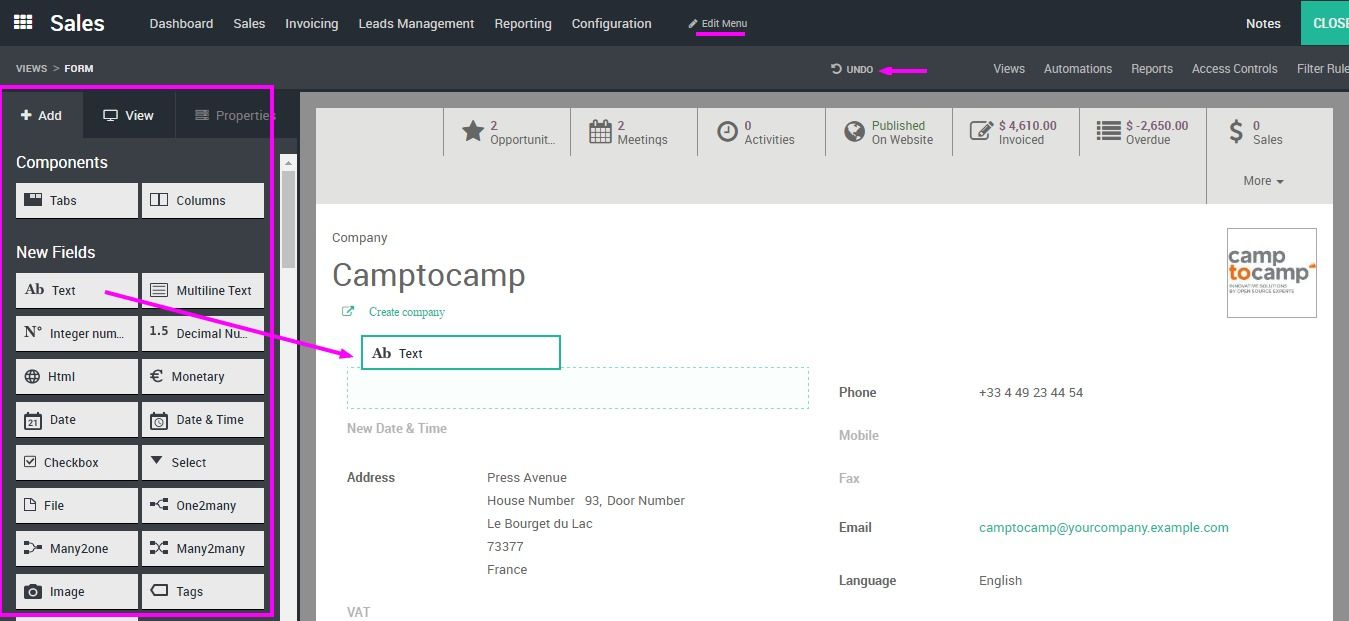
\includegraphics[width=12cm]{../pics/odoo-studio-saas14}
		\caption{\href{https://www.youtube.com/watch?v=xCvFZrrQq7k}{Odoo ``Studio''} is available on the Enterprise and Online versions}
	\end{figure}
}

\frame{
	\frametitle{Support from the Odoo Communication Association (OCA)}
	\begin{figure}	
		\centering
		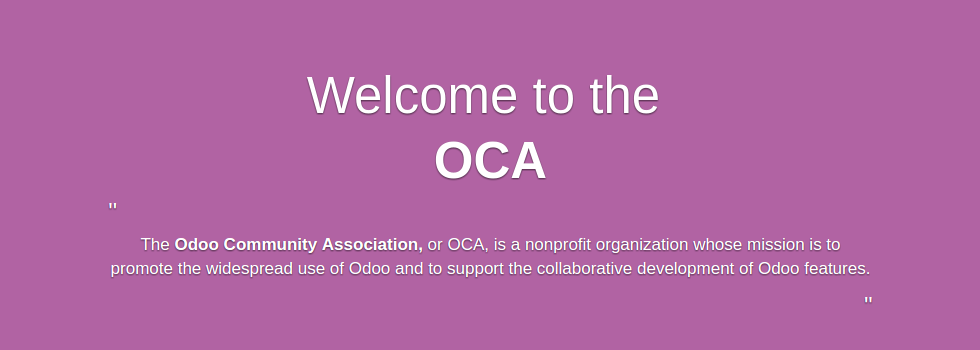
\includegraphics[width=12cm]{../pics/odoo-OCA}
		\caption{\url{https://odoo-community.org} (\cite{oca})}
	\end{figure}
}

\frame{
	\frametitle{Developers love Python}
	\begin{figure}	
		\centering
		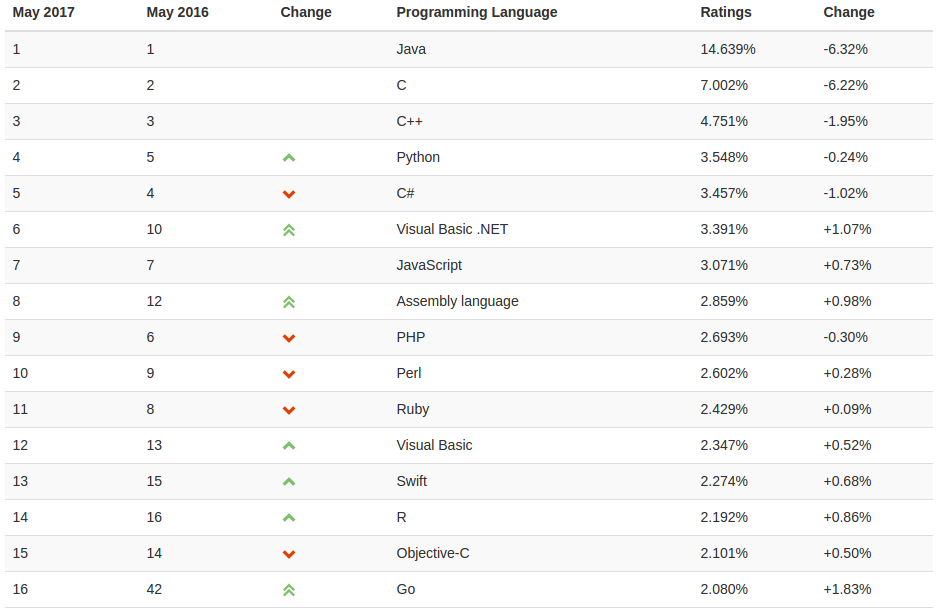
\includegraphics[height=6cm]{../pics/tiobe-index-201705}
		\caption{The \href{https://www.tiobe.com/tiobe-index/}{TIOBE index} shows Python's popularity thrives after 25+ years of existence}
	\end{figure}
}

\frame{
	\frametitle{Thousands of Open Source modules in developer-friendly format}
	\begin{figure}	
		\centering
		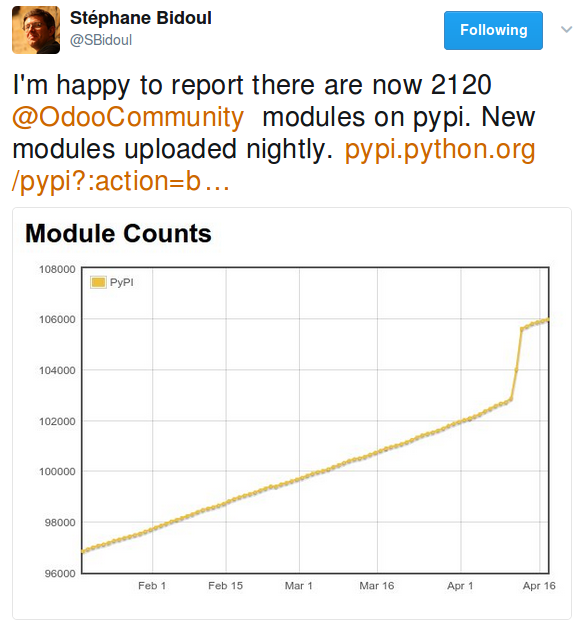
\includegraphics[height=6cm]{../pics/odoo-pypi}
	\end{figure}
}

% ======================================================================================================
%                                     Getting started with Odoo
% ======================================================================================================
\section{How to get started with Odoo}
\subsection{Versions of Odoo}
\frame{
	\frametitle{Versions of Odoo}
	\framesubtitle{Opencore Model}
	\begin{itemize}[<+->]
		\item Odoo Community
			\\{\tiny$\surd$ Open Source, Free, Forever}
		\item Odoo Enterprise
			\\{\tiny$\surd$ added-value Enterprise Modules, run by the Odoo customer, better choice for large and complex deployments}
		\item Odoo Online (aka SaaS)
			\\{\tiny$\surd$ added-value Enterprise Modules, run by Odoo SA, free support, low TCO, less flexibility}
		\item Developer version
			\\{\tiny$\surd$ covered in the workshop portion}
		\item See \url{https://www.odoo.com/pricing} 
			\\and \url{https://www.odoo.com/page/editions} for more details
	\end{itemize}
}

\frame{
	\frametitle{Getting started with Odoo}
	\framesubtitle{Pick your deal}
	\begin{figure}	
		\centering
		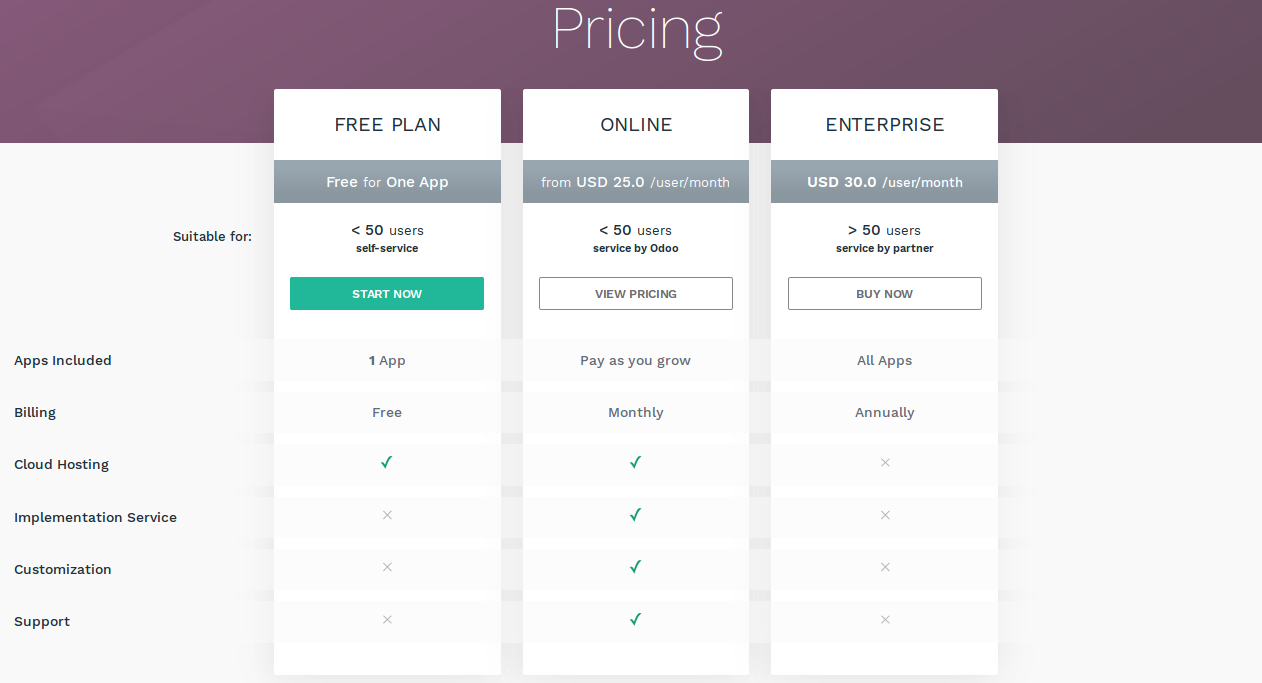
\includegraphics[height=6cm]{../pics/odoo-pricing}
	\end{figure}
}

\frame{
	\frametitle{The free plan is a good place to start}
	\centering
	\Huge{Let's try Odoo!\\\url{https://www.odoo.com/trial}}
}

\frame{
	\frametitle{Experiment with different versions of Odoo}
	\begin{figure}
		\centering
		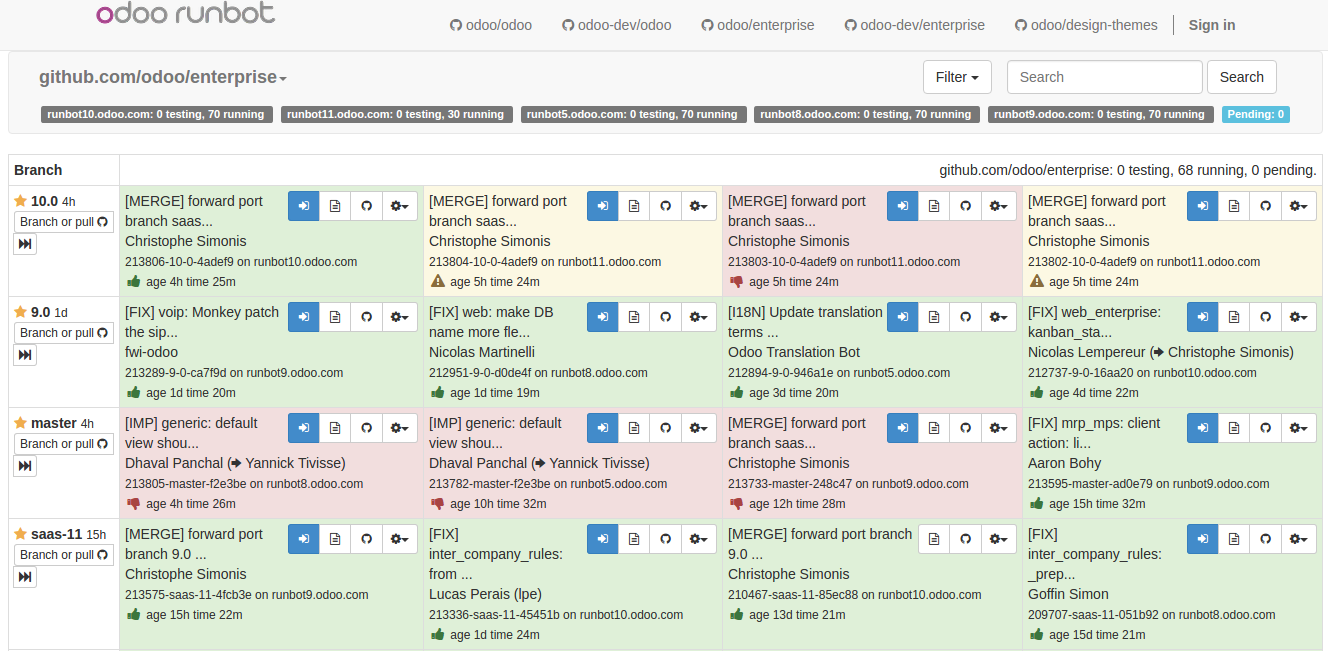
\includegraphics[width=12cm]{../pics/odoo-runbot}
		\caption{\url{http://runbot.odoo.com/runbot}}
	\end{figure}
}

\subsection{Where is Odoo going next?}
\frame{
	\frametitle{The future of Odoo}
	\begin{figure}
		\centering
		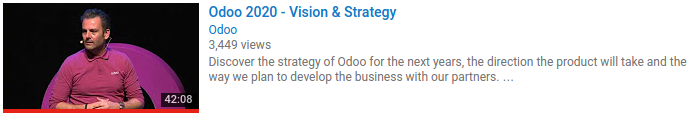
\includegraphics[width=12cm]{../pics/odoo-vision2020}
		\caption{\url{https://www.youtube.com/watch?v=v8eumtr3X1Q}}
	\end{figure}
	\begin{figure}
		\centering
		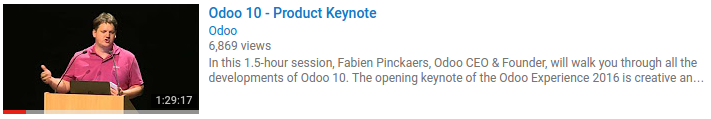
\includegraphics[width=12cm]{../pics/odoo-odoo10keynote}
		\caption{\url{https://www.youtube.com/watch?v=TMno_mDkBRE}}
	\end{figure}
}

% ~ ~ ~ References
% ======================================================================================================
%                                     References
% ======================================================================================================
\section{References}
\frame[allowframebreaks]{
	\frametitle{Odoo: the course ERP}
	\framesubtitle{References}
	% keyword refers to bib file: references-KEYWORD.bib, and to the Tex file: section-KEYWORD.tex
	\printbibliography[keyword=odoo-course-erp]
}

\end{document}

